% Maintain the consistency.
% Maintain a good writing flow. 

\section{Introduction}\label{sec:introduction}
One of the major benefits of using technologies is that it costs less time and instance in most of the cases to perform the same operation than with analog process. Conventionally we still perform all the official tasks through paper work. It not only consumes more time, but also makes students dependent on authority and on specific time period set by the authority. Also, there are always chances of being unsuccessful to complete the process with or without wrong information. In addition, taking attendance manually is also a time-consuming method. Our goal is to develop an application that aims to shift these two process into a digital platform which will obviously be able to perform the given tasks in the shortest time possible with no paper work. The system should be able to let the students get the liberty from the tormenting limitations of the administration and also to let the authority to make their responsibility easier. It goes without saying that the application would be a user-friendly application to both students and authority.

This document objectifies  a recording of a strategic and creative process focused on clearly outlining issues, goals as well as overview of the application representing the narrative from the beginning to the end. Any person willing to use as well as develop the system would be able to do so by the help of this documentation.

The objective of this course is to develop a database application system by applying the theories, methodologies, tools, and technologies we learnt in CSE 413 that is Database System course.  

\clearpage


\subsection{Background and Motivation}\label{subsec:bm}

Since 1966, the establishment of the university, each year the number of students are increasing. Whereas day by day, the world is being introduced with new technologies, the procedure to receive fees and attendance system remained same in University of Chittagong. Being dependent on one specific branch of an individual bank, the payment system of fees has become troublesome not only to the students but also to the administration. Students find this analog system dreadful while they are binded with a time period of a day to submit the fee during class days or a time near the examination. University Authority as well as bank authority have been seemed to be tired of this miserable process as the number of students has a positive growing rate each year. Same goes for the traditional attendance system. Teachers have been recorded to bestow 25 to 30 percentage of a class period to attest the attendance conventionally.

If we look closely, these problems are related to each other. We intend to develop a system that can solve these problem while processing with some basic data of both students and teachers. The system will requires no paper work and least possible physical presence of authority as well as students to perform the operations. Both payment and attendance system will become an one click process throughout the development of the application. Administrations will find it easier to query the needed information than ever before. Students as well as administration may operate the processes from anywhere at anytime with an instant time in this application.

\subsection{Problem Statement}\label{subsec:ps} 

\emph{To develop a database system that can be used to handle payment system of fees of student and attendance system online.}

The system will be using student data such as \emph{name}, \emph{student id}, some institutional data such as \emph{course}, \emph{department}, some teacher's data such as \emph{teacher's name}, \emph{the department he belongs to} and \emph{which courses he teaches} and so on. The system will also hold the records of payments already done or have to be done by a student. With the information of courses from a teacher and the students studying the course, the attendance system will be implemented in the same application.

\clearpage

\subsection{System Definition}\label{subsec:sd} 

\textit{``An online application used to handle the payment system of fees by the students and attendance system. The application should transform and shift the analog payment system into digital platform and prevent the time-consuming process."}


\subsection{System Development Process}\label{subsec:sdp}

There are several phases for a software development life Cycle (SDLC). Requirement gathering and analysis is the foremost and most important phase among them. During this phase, the client expresses the expectations of the project including who will use the product, how the customer will use the product, and the particular data included with any exceptional client requirements identified with the product. To accumulate prerequisites, project administrators ordinarily utilize a few methods. Interviews, surveys, observations, workshops are the most widely recognized of them. Determined to assemble requirements, we used to interview and questionnaire techniques.\\

\begin{figure}[H]
    \centering
    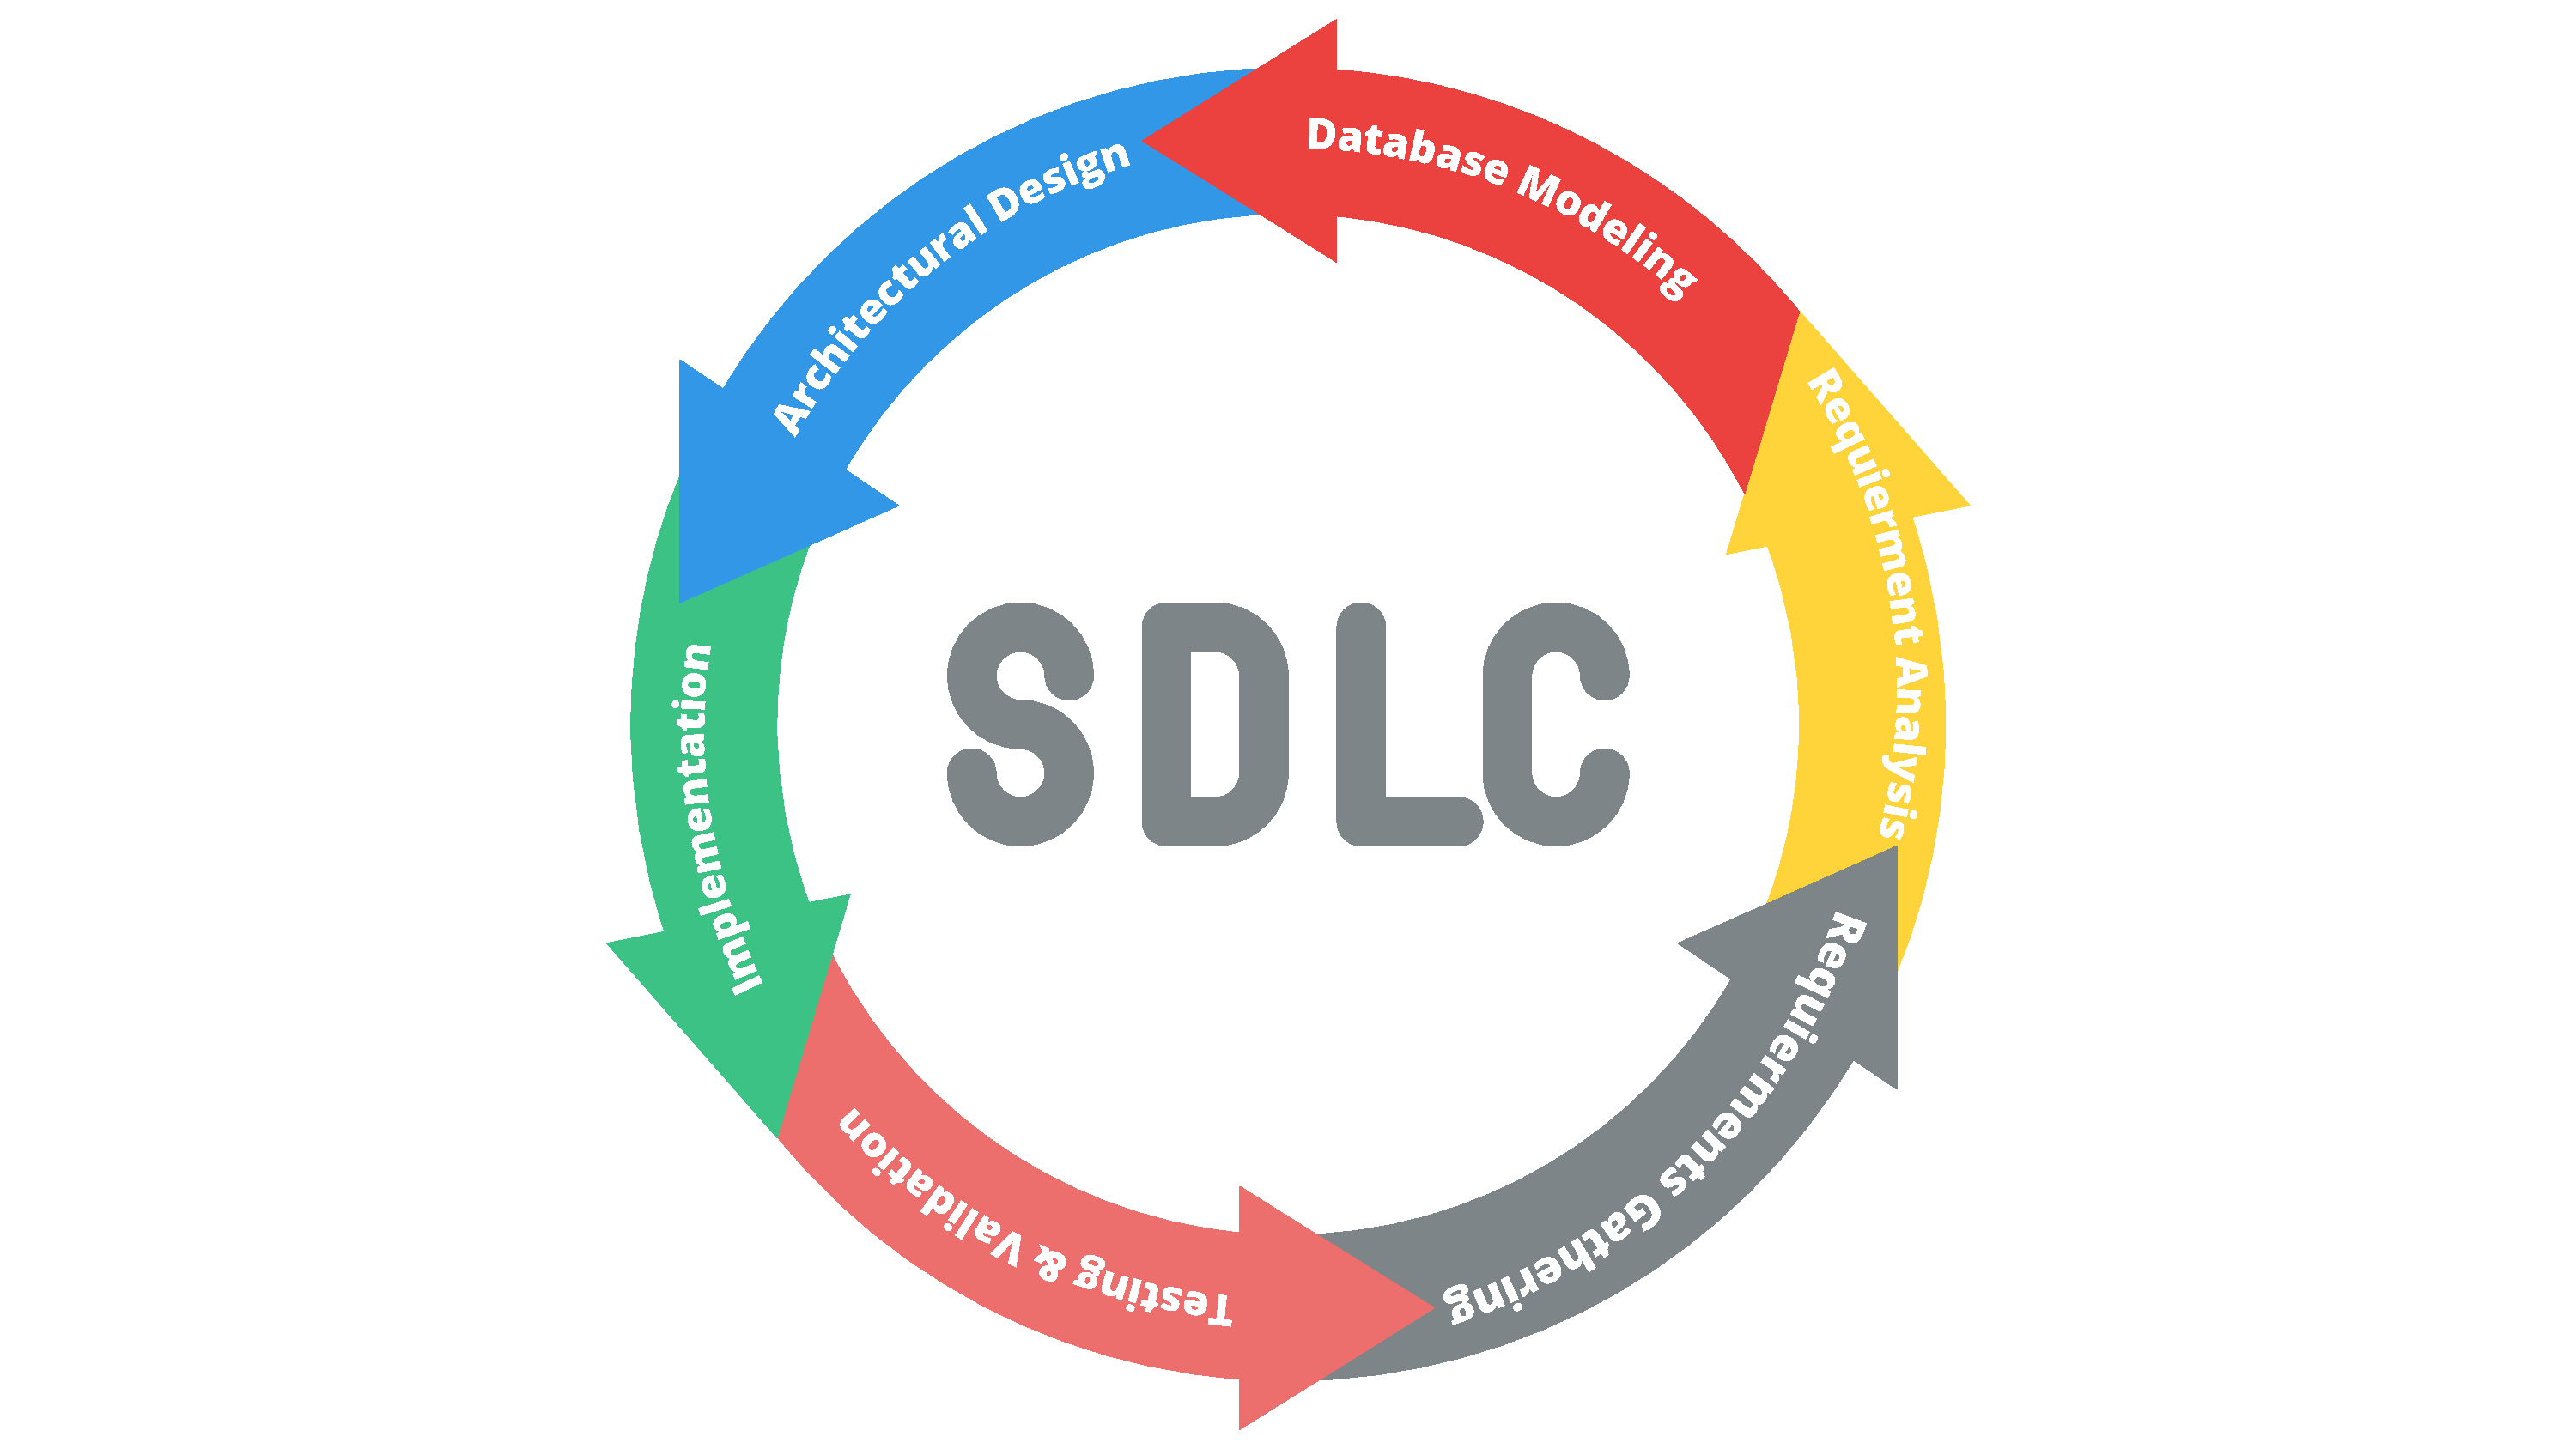
\includegraphics[width=1\textwidth]{images/sdlc}
    \caption{Software Developement Life Cycle (SDLC)}
    \label{fig:sdlc}
\end{figure}

Requirements investigation is critical and fundamental movement later requirement assembled. We break down, refine, and investigate the assembled requirements to make predictable and unambiguous necessities. This movement audits all requirements and may give a graphical perspective on the whole framework. Later the consummation of the examination, it is normal that the understandability of the task might improve essentially. Here, we may likewise utilize the connection with the client to explain points of disarray and to comprehend which requirements are a higher priority than others.\\

Database modeling also called data modeling, is the process of creating a data model for the data to be stored in a database.  It is the third phase of SDLC. This data model is a conceptual illustration of data objects, relationships between them, and the rules.  The Data Model is characterized as a theoretical model that arranges information depiction, information semantics, and consistency limitations of the information. The information model underlines what information is required and how it ought to be coordinated rather than what tasks will be performed on information.\\

There are basically three types of data models. These are conceptual data models, logical data models, and physical data models,  each with a specific purpose.\\

\begin{itemize}
  \item The conceptual data model mainly defines what the system contains. This model is commonly created by business stakeholders and Data Architects. The intention is to put together, scope, and characterize business ideas and rules.
  \item The logical data model defines how the system should be implemented independently of the DBMS. This model is regularly made by Data Architects and Business Analysts. The object is to foster a specialized guide of rules and information structures.
  \item The physical data model depicts how the system gonna be implemented using a particular DBMS. This model is commonly made by DBA and engineers. The intention is the actual implementation of the database.
\end{itemize}

System architecture is an illustrative design that depicts the structure of a system. It contains all the components of the system including subsystems that completely address the functionalities of the system. CU-OPAS is a web-based application system that works with request-response patterns. Using the frontend user interface, any authentic user of this system can request queries regarding payment and attendance operation to the backend API. Then the backend API interacts with the database server and generates a response according to queries that are sent back to the frontend.\\
\begin{figure}[H]
    \centering
    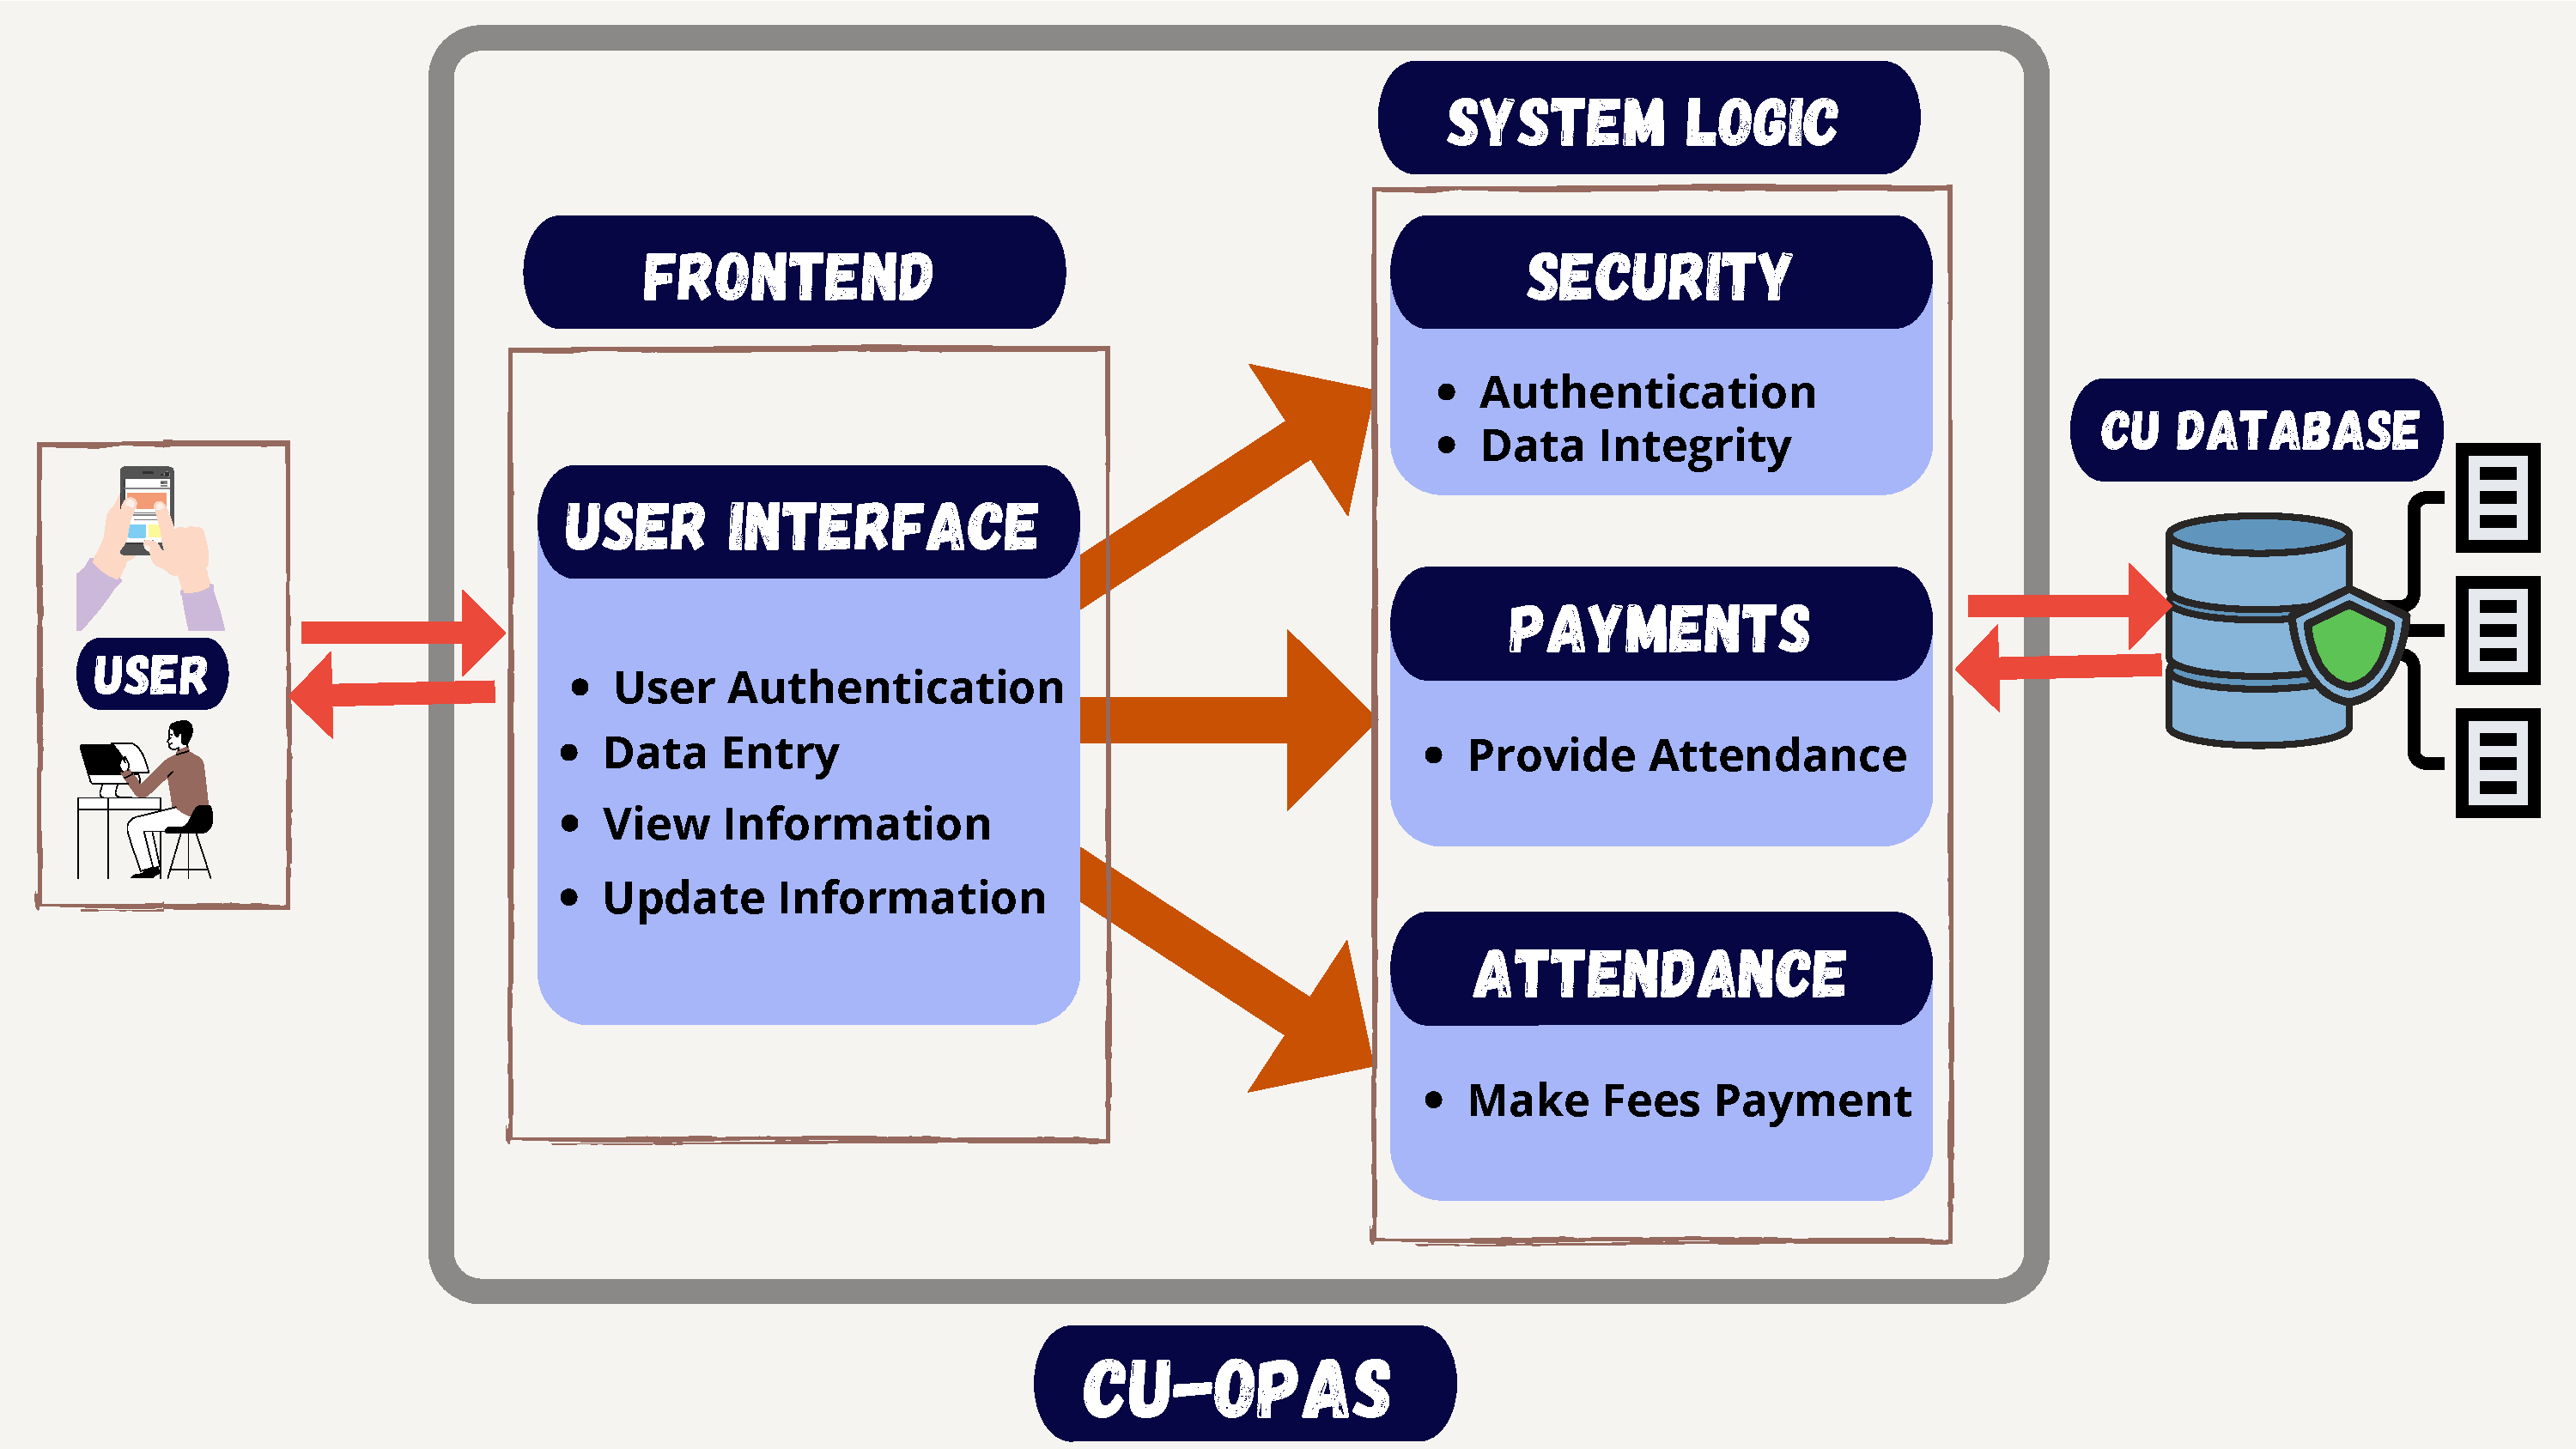
\includegraphics[width=1\textwidth]{images/archi}
    \caption{Architectural design of CU-OPAS}
    \label{fig:archi}
\end{figure}

After successfully completing the architectural design and user testing, implementation begins. The physical design of the system takes place in this phase. It is the SDLC's third phase. During this phase, we used a variety of programming languages, frameworks, tools, and internet resources to build our system.\\

The final and most crucial phase of the SDLC is validation. This step is critical in ensuring that not just the proper product, but also a high-quality product is produced. Validation can determine whether or not the system meets end-user requirements. We've tested our system in a variety of ways for this aim, including Unit Testing, Integration Testing, System Testing, and Acceptance Testing.
\begin{comment}


To design a database, one should follow the following steps:
\begin{enumerate}
\item Requirement analysis
	\begin{itemize}
		\item[-] interviewing, documentation, etc .
	\end{itemize}

\item Mapping onto a conceptual model (conceptual design)
     \begin{itemize}
     	\item[-] ER model
     \end{itemize}
\item Mapping onto a data model (logical design)
	\begin{itemize}
     	\item[-] Relational model, object model etc. 
     \end{itemize}
\item Normalization
\item System Architecture
\item Realization and Implementation (physical design)    
    
\end{enumerate}
\end{comment}


\subsection{Organization}
Section~\ref{sec:introduction} gives an overview of this project. this section also narrates the project from start to the end briefly. Section~\ref{sec:projectmanagement} describes how the project and the resources are managed. The next section~\ref{sec:rga} refers to the results of the analysis of the information gathered from the surveys, interviews and discussion with some group of students, teachers and administrative officers. The following section~\ref{sec:cm}, section~\ref{sec:lm} and section~\ref{sec:norm} gives the overview of how we designed the database and enhanced it step by step as most as possible. Section~\ref{sec:sa} and section~\ref{sec:imp} gives the information about the whole system structure and how we implemented it. Section~\ref{sec:val} says how we validated the system with real user data with an statistics on consumed time, cost, user satisfaction between the previous system and this system. Section~\ref{sec:sd} is about the process to install and configure the system so that even a non-technical person can use the system easily. Finally, the conclusion and the pointers to the future work are outlined in Section~\ref{sec:cfw}.

\clearpage